\section{Experiments}
\label{sec:experiment}
In this section, we conduct experiments on three real-world news datasets: 
Adressa~\cite{gulla_adressa_2017}, Globo~\cite{moreira_news_2018} and MIND~\cite{wu2020mind}. 

\subsection{Experimental Setup}
\subsubsection{Data Preprocessing}
In dataset preprocessing, we treat a series of click events from one anonymous user 
within 30 minutes as a session. 
We discard the sessions no longer than 1 click.
To augment limited training data, for a session of $n$ clicks, we create $n-1$ mini-sessions, 
each starting from the first click of the original session and ending at the 2nd, 3rd through
the last click of the original session. The article clicked at the end of every mini-session is 
the label to be predicted. The dataset statistics are 
in \tabref{tb:dataset}, where each session is quite short. We only choose a subset of days 
in Adressa (the whole dataset lasts for 3 months) following~\citet{moreira_contextual_2019} 
for simplicity, and as for MIND, the data from the first several weeks is 
the historical logs without the session information, so we choose the data from the last week.

\begin{table}[th]\setlength{\tabcolsep}{2.7pt}
  \caption{Dataset statistics (after preprocessing)}
  \label{tb:dataset}
  \centering
  \begin{tabular}{l|cccccccc}
    \toprule
    % \multicolumn{2}{c}{Part}                   \\
    % \cmidrule(r){1-2}
     Dataset & \tabincell{c}{\# \\sessions} & \tabincell{c}{\# \\articles} & \tabincell{c}{\# \\topics}&\tabincell{c}{clicks\\/session}  & \tabincell{c}{clicks\\/article} & \tabincell{c}{Days\\covered}\\
    \midrule
    Globo & 1M & 45k & 461 & 2.69 & 64 & 16 \\
    Adressa & 0.5M & 12k & 23 & 2.79 & 117 & 20 \\
    MIND & 0.2M & 7k & 16 & 2.38 & 59 & 7 \\
    \bottomrule
  \end{tabular}
\end{table}

\subsubsection{Train/test set split}
In order to simulate the real-time recommendation 
scenario, we train the model in the first few days and test the trained model in the remaining
days~\cite{jugovac_streamingrec:_2018}. Each dataset can be split into several folds, 
we will average the results over these folds.
%for Globo dataset, we split every 4 days into one fold, with 3 day for training and 1 day for testing, and 4 folds in total. For Adressa dataset, we split every 10 days into one fold due to its fewer session data in one day. We average metrics performance of each folds in the end. For MIND dataset, we leave the last day as test. 
After data augmentation, the ratio between training data size and test data size 
is around 6:1 for Globo, and 10:1 for the other two datasets. 

%\begin{figure}[th]
%  \centering
%  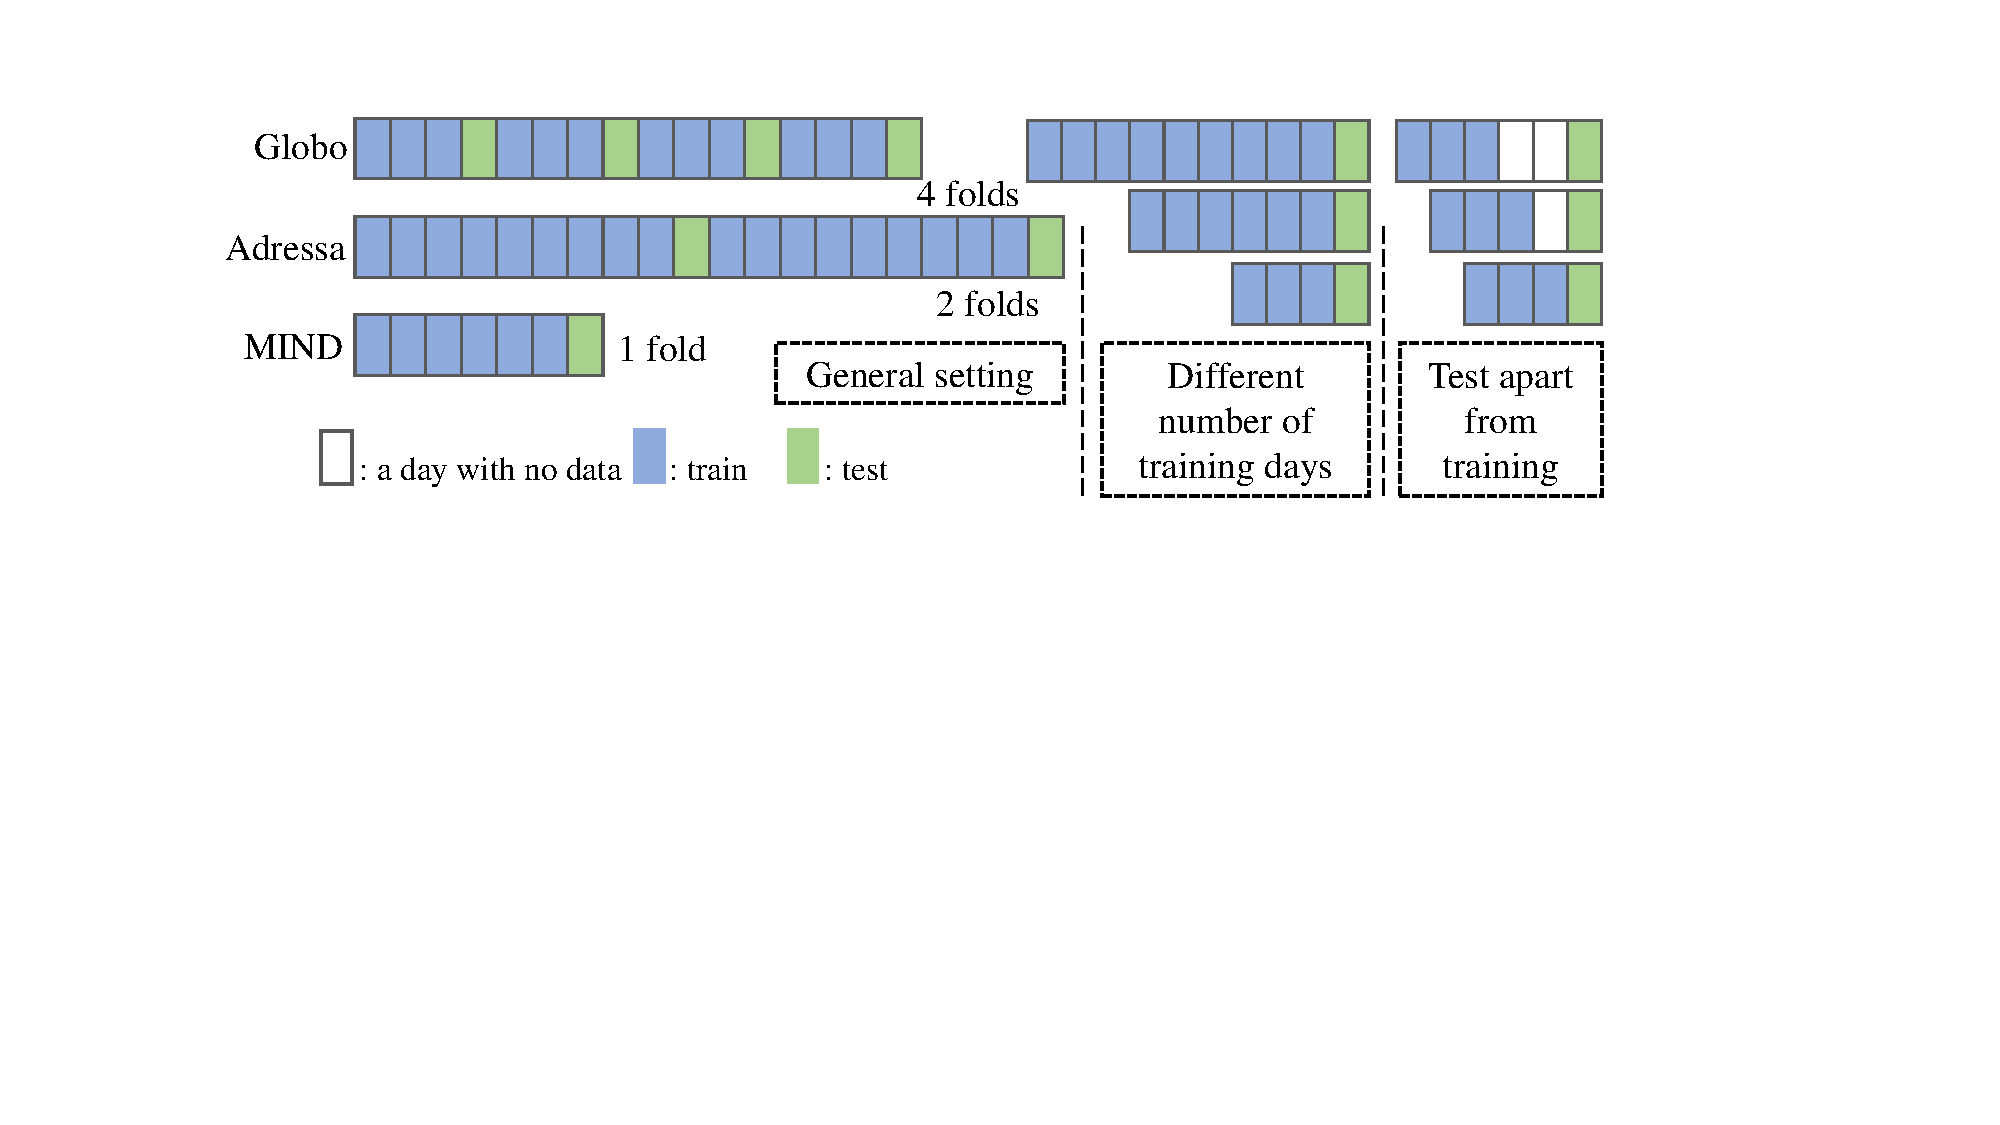
\includegraphics[width=\columnwidth]{fig/data_split.pdf}
%  \caption{Dataset splits to simulate different scenarios.}
%  \label{fig:data_split}
%  \Description[Data split]{An illustration of train/test set split.}
%\end{figure}

\subsubsection{Metrics}
During the test, given the first few click events in a session, the model generates 
a top-$k$ recommendation list $R$ with descending probabilities. 
We use widely-used metrics HR@k (Hit Rate), NDCG@k (Normalized Discounted Cumulative Gain) to 
measure the model's prediction accuracy.

Intra List Diversity (ILD@k)~\cite{symeonidis2020session} evaluates the topical/semantic 
diversity in $R$, and reflects the model's ability to recommend different items to the same users. 
\begin{equation}
  ILD@k = \frac{1}{|R|(|R|-1)}\sum_{i\in R}\sum_{j\in R}d(i,j),
\end{equation}
where $d(i, j)$ is a distance measure between items $i$ and $j$, and 
$d(i, j) = 1$ if item $i, j$ belong to different topics (categories).

\subsubsection{Baseline Algorithms}
%For this experiments, an extensive number of session-based recommendation algorithms was used for comparison, sequential modeling algorithms to predict next clicked item are also taken into consideration. Despite of the simplicity of some of those methods, they still have competitive accuracy on session-based recommendations.

\paragraph{Simple approaches without deep learning.}

\textbf{CBCF}~\cite{sottocornola2018session} is a news recommender combines Content-Based similarity with session-based Collaborative Filtering similarity.
\textbf{STAN}~\cite{garg2019sequence} is an extended version of SKNN (Session-KNN) with three controllable temporal decay factors.

\paragraph{Session-based neural recommendation approaches.}
  \textbf{GRU4Rec}~\cite{hidasi2015session,hidasi2018recurrent} is a Gated Recurrent Unit for recommendation, building with gated recurrent neural networks, which is similar to LSTM in ~\cite{moreira_news_2018}.
  \textbf{SASRec}~\cite{kang_self-attentive_2018} is a self-attention based Sequential model, adopting Transformer architecture to model user's action.
  \textbf{STAMP}~\cite{liu2018stamp} is a Short-Term Attention/Memory Priority Model for Session-based Recommendation, introducing the attention mechanism to model the relationship of each historical click and the last click.
  \textbf{SRGNN}~\cite{wu2019session} is a Session-based Recommender using Graph Neural Networks to capture complex transitions of items.
  \textbf{SGNNHN}~\cite{pan2020star} is improved SR-GNN using Star Graph Neural Network.
\paragraph{Neural news recommendation approach.}
\textbf{CPRS}~\cite{wu2020CPRS} is a typical news recommendation approach that utilizes the textual feature of articles to model user's interests. It also uses the dwell time (i.e. active time) to measure user's satisfaction. We make this approach adapt to the session-based scenario.

\subsubsection{Implementation Details}
For fair comparison, we apply all baselines to the same augmented data and train 
models on one GTX1080Ti GPU.
We use the same latent dimensions $d=250$ and choose different learning rate $\{0.01, 0.001, 0.0001\}$, batch size $\{512, 1024, 2048\}$ and other hyper-parameters to select the best model using early stopping strategy based on the HR@20 score on the validation set, which is the last 10\% of samples in the training set sorted by time. All embedding tables are normally initialized with 0 mean, 0.002 standard deviation, and for weighting parameters 0 mean, 0.05 standard deviation.

\subsection{Main Results}
\label{sec:mainres}
\begin{table*}[th]\setlength{\tabcolsep}{2.5pt}
\caption{Main results ($k=20$). All results are averaged over all folds. The best baseline result on 
each metric is marked with $*$ and overall best results are bolded. 
CAR is our base model, and P, N, R are respectively positive feedback, negative feedback, 
random negative sampling. The last column is our whole model. 
$\uparrow$ indicates improvement over the base model.}
  \label{performance-table}
  \begin{threeparttable}
  \centering
  \begin{tabular}{p{1.2cm}<{\centering}p{1.1cm}<{\centering}|p{0.8cm}<{\centering}p{0.8cm}<{\centering}p{1.2cm}<{\centering}p{1.2cm}<{\centering}p{1.2cm}<{\centering}p{1.3cm}<{\centering}p{1.1cm}<{\centering}|p{1.1cm}<{\centering}p{1.1cm}<{\centering}p{1.1cm}<{\centering}p{1.1cm}<{\centering}p{1.1cm}<{\centering}}
  \toprule
  Datasets&Metrics&CBCF&STAN&GRU4Rec&SASRec&SRGNN&SGNNHN&STAMP&CAR&CAR+P&CAR+N&CAR+R&Whole \\ 
  \midrule
  \multirow{3}{*}{Adressa} & HR & 0.0957 & 0.1130 & 0.1120 & 0.1205 & 0.1152 & 0.1186 & 0.1287$^*$ & 0.1436 & 0.1532$\uparrow$ & 0.1518$\uparrow$ & 0.1455 & \textbf{0.1643} \\ 
  \cline{2-14}
  & NDCG & 0.0341 & 0.0500 & 0.0511 & 0.0509 & 0.0536 & 0.0517 & 0.0575$^*$ & 0.0649 & 0.0692$\uparrow$ & 0.0656$\uparrow$ & 0.0645 & \textbf{0.0674} \\ 
  \cline{2-14}
  & ILD & 0.7732 & 0.2409 & 0.8170 & 0.7856 & 0.8611$^*$ & 0.8236 & 0.8445 & 0.8473 & \textbf{0.8631}$\uparrow$ & 0.8325 & 0.8447 & 0.8456\\ 
  \midrule
  % \cline{1-14}
  \multirow{3}{*}{Globo} & HR & 0.1185 & 0.1273 & 0.1280 & 0.1409 & 0.1280 & 0.1439$^*$ & 0.1435 & 0.1340 & 0.1382$\uparrow$ & 0.1402$\uparrow$ & 0.1382 & \textbf{0.1447}\\ 
  \cline{2-14}
  & NDCG & 0.0474 & 0.0647 & 0.0599 & 0.0620 & 0.0627 & 0.0688 & 0.0698$^*$ & 0.0656 & 0.0693$\uparrow$ & 0.0688$\uparrow$ & 0.0683 & \textbf{0.0731}\\ 
  \cline{2-14}
  & ILD & 0.3874 & 0.3043 & 0.9377 & \textbf{0.9864}$^*$ & 0.9248 & 0.9545 & 0.7980 & 0.8154 & 0.8269$\uparrow$ & 0.6427 & 0.8239 & 0.8540\\ 
  \midrule
  % \cline{1-14}
  \multirow{3}{*}{MIND} & HR & 0.0315 & 0.0312 & 0.0338 & 0.0355 & 0.0334 & 0.0366 & \textbf{0.0371}$^*$ & 0.0370 & - & 0.0363 & 0.0365 & 0.0363\\ 
  \cline{2-14}
  & NDCG & 0.0110 & 0.0142 & 0.0132 & 0.0139 & 0.0144 & 0.0122 & 0.0150$^*$ & 0.0147 & - & 0.0154$\uparrow$ & 0.0140 & \textbf{0.0154}\\
  \cline{2-14} 
  & ILD & 0.7166 & 0.3193 & 0.8662 & 0.8562 & 0.8706 & 0.8775$^*$ & 0.8452 & 0.8836 & -  & 0.8839$\uparrow$ & 0.8812 & \textbf{0.8839}\\ 
  \bottomrule
\end{tabular}
\end{threeparttable}
\end{table*}

In \tabref{performance-table}, we compare the performance of all baselines and our
approach, and we can make the following observations.

Non-neural methods CBCF and STAN are either considering the content information or the recency of a past session, and their results are comparable to deep learning methods in three datasets. However, they generate recommendation lists with low diversity, mainly because their simple algorithms cannot capture enough personalized information. For session-based approaches, generally speaking, STAMP and SGNNHN yield better performance on HR and NDCG, but not always good at ILD, showing the trade-off between diversity and accuracy. From the user's aspect, though, when ILD is over a threshold (like 0.85), it's hard for them to distinguish the difference. 

As for our whole model, when compared with STAMP, it performs better on both accuracy and diversity 
except for HR score on MIND, but the better NDCG score means it recommends the true article
at a higher rank. This result shows that our model mitigates the dilemma between accuracy and diversity 
to a certain extent. What's more, our model significantly outperforms others in Adressa 
because this dataset provides the most complete information. It not only releases the original 
text of articles instead of the extracted vectors in Globo, but also gives the accurate active time 
of the user in each article, while we can only estimate the active time by the interval between 
two successive clicks for Globo, which may not be accurate. In the MIND dataset, 
the improvement is comparatively small and the possible reasons are: 
on the one hand, MIND didn't provide active interval, nor did they give click time of each article, 
we cannot get positive feedback from the data; on the other hand, from the results of CBCF, 
we assume the article transition information is too sparse and thus hard to recommend. 
Note that this dataset is not designed for the session-based recommendation, thus some information 
may be inaccurate (e.g., the time of a session is longer than 30 minutes).

\subsection{Ablation Analysis}
% \label{sec:abla}
From \tabref{performance-table} we can verify the effects of modeling user positive and negative implicit feedback in our model. Compared with the base model, there is significant improvement after adding $P$ and $N$ modules and this improvement is consistent for positive feedback modeling. It's because that the negative samples from the impression list are reconstructed based on their publish time, so the information is not totally reliable. To verify the effect of the negative sampling strategy more accurately, we set the control group with random sampling, and we find that even though the random sampling would increase or decrease the performance slightly, our negative feedback shows superior performance over it. 
The table also shows that adding $N$ module lowers diversity, possibly because that in the datasets the negative samples and the positive article usually belong to different categories, thus adding $N$ forces the model to recommend similar articles to the positive one.

\subsection{The Modeling of Positive Feedback}
CPRS considers the active time to represent the user's satisfaction using personalized reading speed, which is quite similar but more complex than our positive feedback modeling. We first modify this method to meet the 
session-based scenario, and second plug the personalized reading speed into our model. 
The experiment is conducted in Adressa due to its complete information 
(Globo does not provide the text-level content and the active time is missing for MIND). 
In \tabref{tb:CPRS}, the poor score of CPRS shows that when it is adapted to the session-based scenario, 
limited interactions are the bottleneck. When we adopt their personalized reading speed instead of 
the reading time, there is no significant improvement, and we hypothesize that for this dataset, 
in news reading the reading speed is quite similar for different users.

\begin{table}[th]\setlength{\tabcolsep}{3pt}
  \caption{Results of CPRS and CPRS module plugged into our model in Adressa dataset.}
  \label{tb:CPRS}
  \centering
  \begin{tabular}{c|ccc|c|ccc}
    \toprule
    % \multicolumn{2}{c}{Part}                   \\
    % \cmidrule(r){1-2}
    \multirow{2}{*}{CPRS}& HR & NDCG & ILD & \multirow{2}{*}{\tabincell{c}{Ours w/\\CPRS}} & HR & NDCG & ILD\\
    \cline{2-4}\cline{6-8}
    &0.0812 & 0.0371 & 0.8191 & & 0.1641 & 0.0674 & 0.8457\\
    \bottomrule
  \end{tabular}
\end{table}

\subsection{Hyper-parameter Analysis}
We further conduct a parameter analysis on loss weights $\lambda$ and the number of negative samples $|Ne|$ 
in \eqnref{eq:loss}. We report results on Adressa as an example, and results from other datasets are similar. 
The number of negative samples does not matter much, as shown in \figref{fig:para_a}, 
so for simplicity we choose $|Ne|=20$. The performance gets worse if $\lambda$ is set too low or too 
high in \figref{fig:para_b}, we conclude that the negative loss is useful but too many weights on it will harm the learning of the user's positive feedback.
% \begin{figure}[th]
%   \centering
%   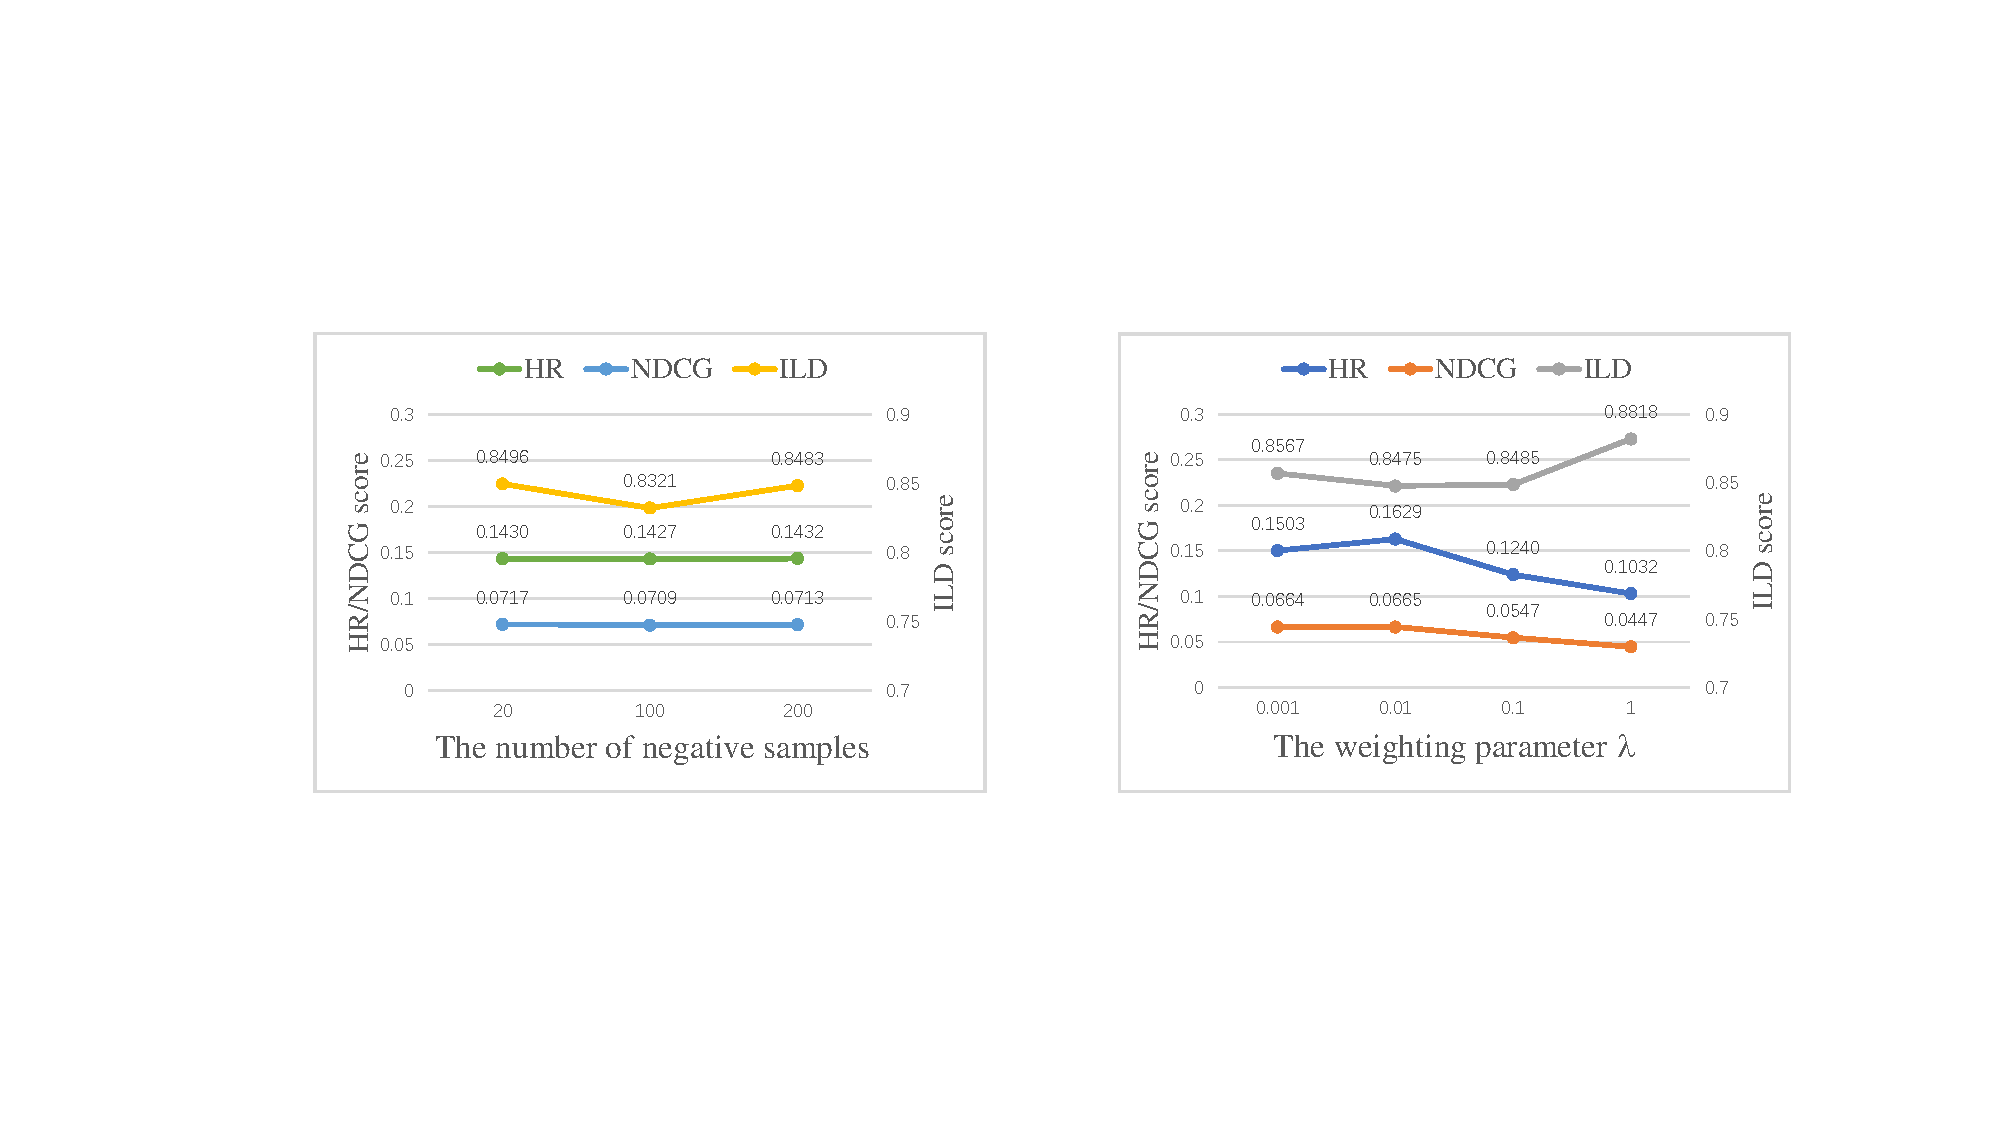
\includegraphics[width=0.95\columnwidth]{fig/parameter.pdf}
%   \caption{Results on different hyper-parameters, which are respectively conducted in Globo and Adressa dataset. \KZ{Make these two subfigs so we can arrange them freely. Make the fonts 
% bigger and darker. I suggest you plot with gnuplot instead of excel, which looks no so nice.
% I also don't get it why the x label on both figs are different? Aren't these two figs
% for Globo and Adressa respectively? Why they measure diff things?}
%   % A user may spend different amounts of time on different clicked articles, refering to different degrees of the implicit positive feedback, and the unclicked articles within/without impression list of the user also show different degrees of the implicit negative feedback. 
% }
% \label{fig:session}
% \end{figure}

\begin{figure}[ht]
  \begin{subfigure}{.235\textwidth}
    \centering
    % include first image
    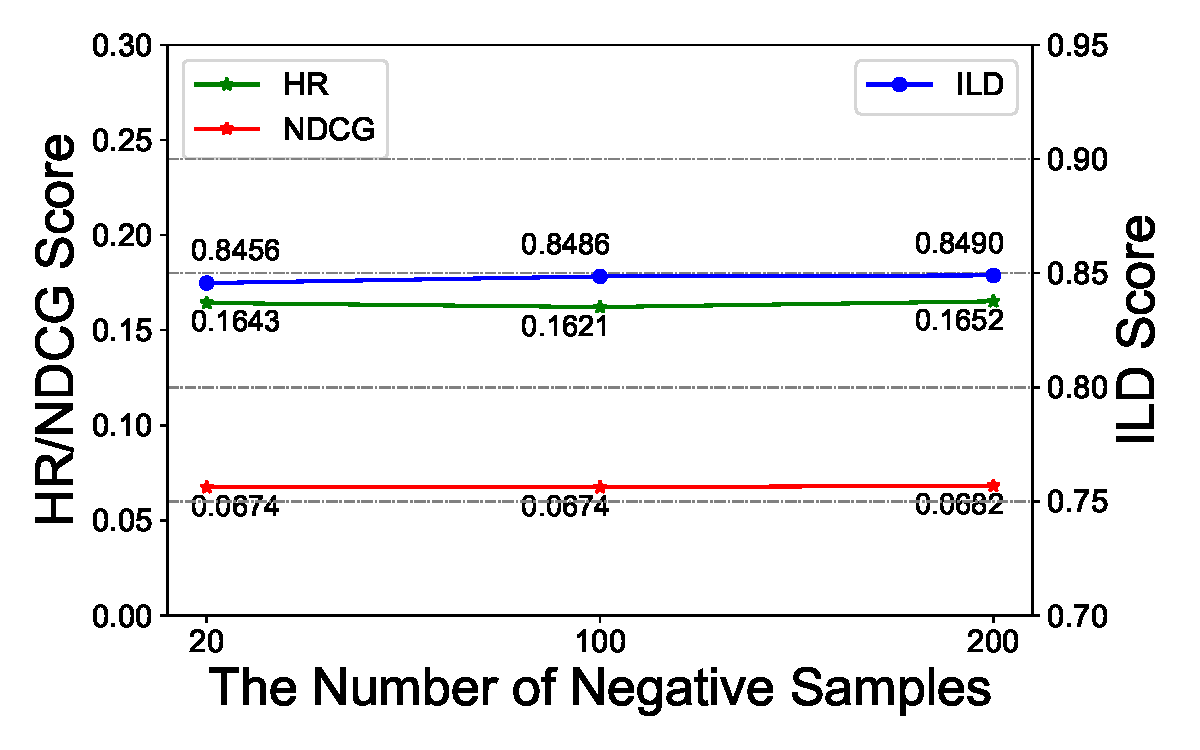
\includegraphics[width=\linewidth]{fig/parameter_a.pdf}  
    \caption{Results for different $|Ne|$.}
    \label{fig:para_a}
  \end{subfigure}
  \begin{subfigure}{.235\textwidth}
    \centering
    % include second image
    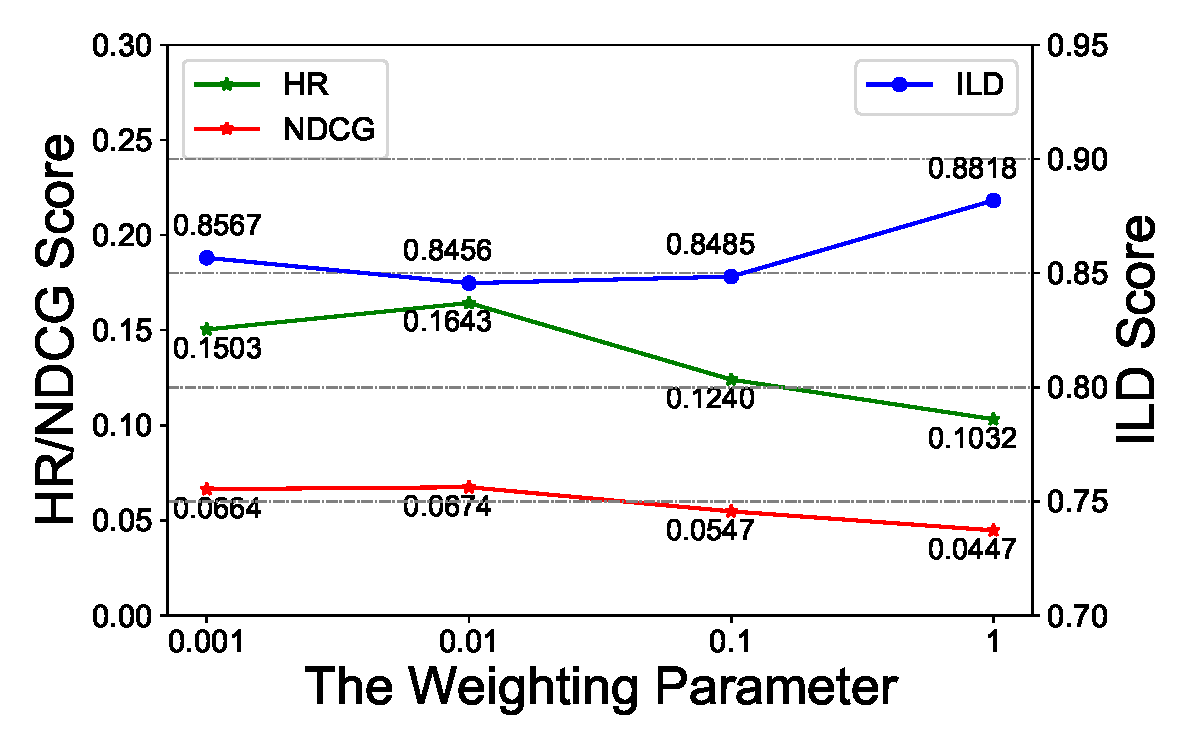
\includegraphics[width=\linewidth]{fig/parameter_b.pdf}  
    \caption{Results for different $\lambda$.}
    \label{fig:para_b}
  \end{subfigure}
  \caption{Analysis on different hyper-parameters.}
  \label{fig:para}
\end{figure}

% \subsection{Discussion}
% \label{sec:discuss}
% We present some discussion on (i) the performance on user cold-start; 
% (ii) the performance on article cold-start; (iii) the effect of the length of
% training days and the gap between training days test days on the results; and 
% (iv) A verification about the assumption of generating impression lists.
% % \tabref{tb:cold}
% %
% \subsubsection{Inferring user impressions from user clicks}
% In this section, we validate our assumption for the negative user feedback,
% which is articles whose publish time is close to the clicked articles are
% likely presented to the user, or within their impressions.
% We do that with the MIND dataset, in which the real impressions, click times and 
% publish times of articles are all available for all the sessions. 
% We compute the span of the publish times of all the articles in
% each session's impression list, including those articles that are clicked. 
% We call this \textit{impression time span}.
% We find that 63\% of the sessions in MIND have an impression time span of under
% one hour. Only 23\% of the sessions have an impression time span of over 12 hours.
% This shows that users typically only browse news articles that are created within a small 
% time window and click some of them.

